\documentclass[11pt,a4paper]{article}
\usepackage[margin=2.2cm]{geometry}
\usepackage{graphicx}
\usepackage{booktabs}
\usepackage{subcaption}
\usepackage{amsmath}
\usepackage{amssymb}
\usepackage{microtype}
\usepackage{hyperref}
\usepackage{xcolor}
\usepackage{float}
\usepackage{listings}
\usepackage{tikz}
\usetikzlibrary{arrows.meta,positioning,shapes.geometric,fit,backgrounds,calc}

\definecolor{codebg}{RGB}{245,245,245}
\definecolor{codekw}{RGB}{0,90,160}
\definecolor{codecmt}{RGB}{100,120,100}
\definecolor{codestr}{RGB}{150,60,60}
\definecolor{mBlue}{RGB}{52,103,188}
\definecolor{mGreen}{RGB}{56,142,60}
\definecolor{mOrange}{RGB}{230,120,40}
\definecolor{mPurple}{RGB}{120,70,170}
\definecolor{mRed}{RGB}{200,60,60}
\definecolor{mGray}{RGB}{110,110,110}

\lstset{
  basicstyle=\ttfamily\footnotesize,
  backgroundcolor=\color{codebg},
  keywordstyle=\color{codekw}\bfseries,
  commentstyle=\color{codecmt}\itshape,
  stringstyle=\color{codestr},
  showstringspaces=false,
  breaklines=true,
  frame=single,
  framesep=3pt,
  rulecolor=\color{codebg},
  numbers=left,
  numberstyle=\tiny\color{mGray},
  xleftmargin=1.2em,
  language=C++,
  morekeywords={cv,dod,Point2f,Rect,Mat,KeyPoint,DMatch,SIFT,BFMatcher,Size,
                TrackedPoint,size_t,auto,nullptr,float,int,double,bool,void}
}

\title{\vspace{-1.5em}Feature Tracking and Dynamic Object Detection \\
\large A friendly walk-through of the method and the code}
\author{Mahdi Gheysari \and Filippo Businaro \and Riccardo Pesce}
\date{April 2026}

\begin{document}
\maketitle
\vspace{-2em}

\begin{abstract}
This is the long version of our report, written in plain English.
If the two-page report is the \emph{what} and \emph{why}, this one is
the \emph{how}. We explain every step of the pipeline, show the
actual code, and point out who wrote which file. The math and the
parameter choices are all still here --- we just stopped pretending
that our code is a research paper.
\end{abstract}

\tableofcontents
\vspace{1em}

\section{What are we trying to do?}

You get a short video (a folder of numbered frames). Somewhere in
that video, \emph{one thing} is moving --- a bird, a car, a frog, a
sheep, or a squirrel. Everything else is background. Our job is to
look at the \textbf{first frame} and draw a box around that moving
thing.

We cannot use deep learning. Only classical computer vision: corner
detectors, feature descriptors, matching, clustering, geometry. The
dataset gives us five categories, one ground-truth box per category.
We are graded on \emph{Intersection-over-Union} (IoU) between our
box and the ground truth. IoU $\geq 0.5$ counts as a true positive.

\paragraph{What we noticed about the data.} Before writing any code,
we just \emph{looked} at the videos:

\begin{itemize}\itemsep2pt
\item In \textbf{bird}, \textbf{frog}, \textbf{sheep}, and
  \textbf{squirrel}, the camera barely moves. It is sitting on a
  tripod. Only the animal moves.
\item In \textbf{car}, the camera does a slow left-to-right pan.
  The whole scene drifts a little in the same direction.
\end{itemize}

This is important because it tells us we don't need a fancy model of
camera motion. We just need to remove a small, constant drift.

\section{The idea, in plain English}

Here is the whole trick in one sentence:

\begin{quote}
\emph{If you pick some interesting points on the first frame and try
to find them again in every later frame, the background points will
all move together (or not at all), and the object's points will
stand out by moving differently.}
\end{quote}

So the plan is:

\begin{enumerate}\itemsep2pt
\item Put dots on interesting corners of every frame.
\item For each dot on frame 0, find the same dot in every later
  frame.
\item Figure out the ``average'' movement --- that's the camera.
\item Subtract the camera movement. Whatever is left is real object
  motion.
\item Dots with a lot of leftover motion are on the moving object.
  Group them. Draw a box around them.
\end{enumerate}

That's the entire method. The rest of this document is just
explaining what ``interesting corner'', ``find the same dot'',
``group them'', etc.\ actually mean in code.

\section{The big picture}

\begin{figure}[H]
\centering
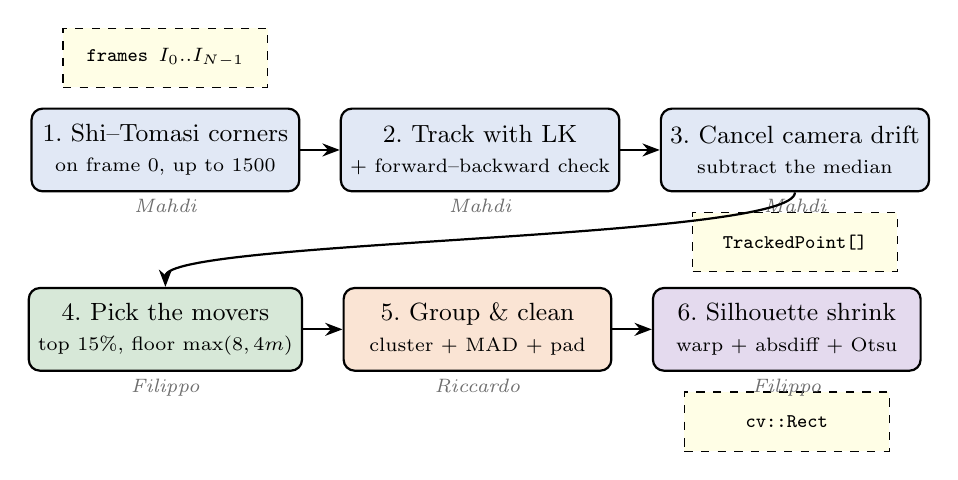
\begin{tikzpicture}[
    node distance=0.45cm and 0.5cm,
    stage/.style={rectangle, rounded corners=4pt, draw, thick,
                  minimum width=3.4cm, minimum height=1.05cm,
                  align=center, font=\small},
    data/.style ={rectangle, draw, dashed, minimum width=2.6cm,
                  minimum height=0.75cm, align=center,
                  font=\scriptsize\ttfamily, fill=yellow!10},
    owner/.style={font=\scriptsize\itshape},
    arr/.style  ={-{Stealth[length=2.2mm]}, thick}
]
\node[stage, fill=mBlue!15]   (s1) {1.~Shi--Tomasi corners\\{\scriptsize on frame 0, up to 1500}};
\node[stage, fill=mBlue!15, right=of s1] (s2) {2.~Track with LK\\{\scriptsize + forward--backward check}};
\node[stage, fill=mBlue!15, right=of s2] (s3) {3.~Cancel camera drift\\{\scriptsize subtract the median}};

\node[stage, fill=mGreen!20, below=1.2cm of s1] (s4) {4.~Pick the movers\\{\scriptsize top 15\%, floor $\max(8,4m)$}};
\node[stage, fill=mOrange!20, right=of s4]      (s5) {5.~Group \& clean\\{\scriptsize cluster + MAD + pad}};
\node[stage, fill=mPurple!20, right=of s5]      (s6) {6.~Silhouette shrink\\{\scriptsize warp + absdiff + Otsu}};

\node[data, above=0.25cm of s1] {frames $I_0..I_{N-1}$};
\node[data, below=0.25cm of s3] {\texttt{TrackedPoint[]}};
\node[data, below=0.25cm of s6] {\texttt{cv::Rect}};

\node[owner, below=-1pt of s1] {\color{mGray}Mahdi};
\node[owner, below=-1pt of s2] {\color{mGray}Mahdi};
\node[owner, below=-1pt of s3] {\color{mGray}Mahdi};
\node[owner, below=-1pt of s4] {\color{mGray}Filippo};
\node[owner, below=-1pt of s5] {\color{mGray}Riccardo};
\node[owner, below=-1pt of s6] {\color{mGray}Filippo};

\draw[arr] (s1) -- (s2);
\draw[arr] (s2) -- (s3);
\draw[arr] (s3.south) .. controls +(0,-0.6) and +(0,0.6) .. (s4.north);
\draw[arr] (s4) -- (s5);
\draw[arr] (s5) -- (s6);
\end{tikzpicture}
\caption{The whole pipeline. Blue = finding and matching points
(\texttt{feature\_tracker.cpp}). Green = deciding which points are
on the object (\texttt{motion\_segmenter.cpp}). Orange = grouping
and boxing (\texttt{bbox\_estimator.cpp}). Purple = optional
silhouette shrink on the pixel-level motion mask
(\texttt{silhouette\_refiner.cpp}). The name under each stage is
whoever wrote it.}
\end{figure}

\section{The method, step by step}

\subsection{What we tried first: SIFT + Lowe's ratio}

Our initial implementation used \textbf{SIFT} keypoints
(\texttt{cv::SIFT::create(1500)}) matched between frame~0 and every
later frame with \texttt{cv::BFMatcher(NORM\_L2)} and \textbf{Lowe's
ratio test} at $0.75$. SIFT is the textbook scale- and
rotation-invariant detector,\footnote{D.~G.~Lowe.
\emph{Distinctive image features from scale-invariant keypoints.}
IJCV, 60(2):91--110, 2004.} and the OpenCV docs ship a tutorial that
is essentially this exact pipeline.\footnote{OpenCV,
\emph{Feature Matching} (4.x),
\url{https://docs.opencv.org/4.x/dc/dc3/tutorial_py_matcher.html}.}

It worked on car and sheep but underperformed on the small or
weakly-textured objects: SIFT scale-invariant extrema do not anchor
reliably on the squirrel's fur or the smooth regions of the frog's
skin, so only $\sim\!13$ tracks ended up tagged dynamic on those
sequences and the resulting bounding box was too small (squirrel
IoU $0.31$, sub-threshold).

The brief gives us another option: \emph{``\dots\ robust feature
matching or \textbf{optical flow} techniques.''} Optical flow
doesn't need a stable scale-space extremum; it only needs a corner
strong enough for Lucas--Kanade to track. So we re-built the
front-end on \textbf{Shi--Tomasi corners + pyramidal Lucas--Kanade},
which is what the rest of this section describes.

\subsection{Step 1 --- Finding interesting points (Shi--Tomasi)}

We need ``interesting'' pixels --- ones we can find again later. A
flat patch of sky is useless; a brick corner is great. The classical
test for ``cornerness'' is the Shi--Tomasi response: at each pixel,
look at the smaller eigenvalue of the local image-gradient covariance
matrix. Points where it's large in both directions are corners.

We use \texttt{cv::goodFeaturesToTrack}\footnote{Docs:
\url{https://docs.opencv.org/4.x/dd/d1a/group__imgproc__feature.html\#ga1d6bb77486c8f92d79c8793ad995d541}.}
on frame~0 with these arguments:

\begin{itemize}\itemsep2pt
\item \textbf{maxCorners = 1500} --- plenty for the cluster stage.
\item \textbf{qualityLevel = 0.005} --- permissive so weak corners on
  textureless surfaces (squirrel fur, frog limbs) still get picked.
\item \textbf{minDistance = 5\,px} --- spatial spread.
\item \textbf{blockSize = 7} --- size of the neighbourhood used to
  compute the covariance matrix.
\end{itemize}

\subsection{Step 2 --- Tracking with Lucas--Kanade}

For every consecutive frame pair $(f-1, f)$ we propagate the
surviving track positions with
\texttt{cv::calcOpticalFlowPyrLK}\footnote{Docs:
\url{https://docs.opencv.org/4.x/dc/d6b/group__video__track.html\#ga473e4b886d0bcc6b65831eb88ed93323}.
Tutorial:
\url{https://docs.opencv.org/4.x/d4/dee/tutorial_optical_flow.html}.
The pyramidal LK algorithm comes from Bouguet, \emph{Pyramidal
Implementation of the Lucas Kanade Feature Tracker}, Intel, 2000.}.
Lucas--Kanade assumes that within a small neighbourhood the
brightness is approximately constant under a single 2D translation
$(u, v)$, and solves for $(u, v)$ from the spatial and temporal
gradients in that window. The pyramidal version repeats the solve at
several down-sampled resolutions so it can handle larger motions
than a single pixel-level pass would.

We use a $21\!\times\!21$ window and $3$ pyramid levels --- the
defaults from the OpenCV tutorial, which is enough for the
inter-frame motion in this dataset.

\paragraph{Forward--backward consistency.} A track that drifts onto
the background, or onto an occluding edge, is a silent failure: the
LK solver returns \emph{some} answer but it's wrong. The standard
filter is to run the flow \emph{backwards} from frame $f$ to
frame $f-1$ starting from the predicted positions, and discard any
track whose round-trip drift exceeds $1.5$\,px. This single check
removes most of the bad tracks and is the same forward--backward
test used in \texttt{cv::TrackerMedianFlow} and Kalal et~al.'s
``forward-backward error'' paper.\footnote{Z.~Kalal, K.~Mikolajczyk,
J.~Matas. \emph{Forward-Backward Error: Automatic Detection of
Tracking Failures.} ICPR 2010.}

\subsection{Step 3 --- Getting rid of the camera's drift}

Imagine the camera pans slightly to the right. Every background
point shifts left by, say, 3 pixels per frame. If we naively
measure displacement we'd say \emph{all} points are moving, which is
useless.

The fix is embarrassingly simple. For each frame $f$, look at the
displacement $\delta_i^{(f)} = p_i^{(f)} - p_i^{(0)}$ of every
matched point and take the \textbf{median} $(\bar m_x, \bar m_y)$.
That's the camera. Subtract it.

\[
\tilde \delta_i^{(f)} = \delta_i^{(f)} - \bar m^{(f)}.
\]

The median is robust\footnote{Same majority-voting idea behind
RANSAC: M.~A.~Fischler and R.~C.~Bolles, \emph{Random sample
consensus}, Communications of the ACM, 24(6):381--395, 1981.
Ours is the single-parameter (pure-translation) special case, so a
median replaces the RANSAC loop.}: even if up to half the matches are on the
object, the other half are on the background and the median still
picks out the background motion. And because four of our five
videos have a static camera, the median is basically zero for those
and subtracting it does nothing --- exactly what you want.

No homography, no RANSAC, no iterative model. Just a median per
frame. This is why the car sequence, which everybody expected to be
the hardest, ends up being our \emph{best} result (IoU 0.78).

\subsection{Step 4 --- Deciding who's on the object}

After steps 1--3 each frame-0 keypoint has two numbers:

\begin{itemize}\itemsep2pt
\item $n_i$: how many frames the track survived (forward--backward
  consistent flow).
\item $r_i$: the total of $\|\tilde \delta_i^{(f)}\|$ across those
  frames --- total ``leftover'' motion after removing camera drift.
\end{itemize}

We compute a single score per point: $\bar d_i = r_i / n_i$, the
average leftover displacement per successful frame. This is the
knob we turn.

We throw out any point with $n_i < 3$ --- not enough evidence. Then
we look at the distribution of $\bar d_i$ across the remaining
points and keep the ones that pass both of these:

\begin{enumerate}\itemsep2pt
\item They're in the \textbf{top 15\%} by score, AND
\item Their score is at least $\max(8\,\text{px}, 4m)$, where $m$ is
  the median of all scores.
\end{enumerate}

\begin{figure}[H]
\centering
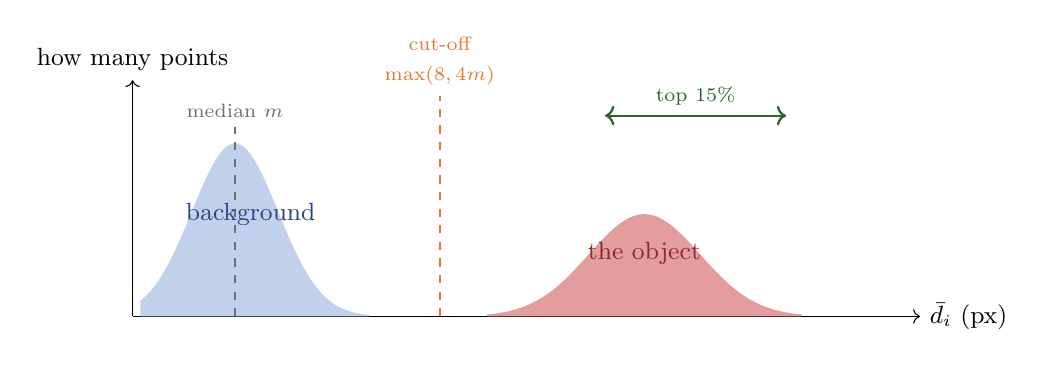
\begin{tikzpicture}[font=\small]
  \draw[->] (0,0) -- (10,0) node[right] {$\bar d_i$ (px)};
  \draw[->] (0,0) -- (0,3) node[above] {how many points};

  \fill[mBlue!30] plot[domain=0.1:3, smooth] ({\x}, {2.2*exp(-(\x-1.3)^2/0.6)}) -- (3,0) -- (0.1,0) -- cycle;
  \fill[mRed!50]  plot[domain=4.5:8.5, smooth] ({\x}, {1.3*exp(-(\x-6.5)^2/1.0)}) -- (8.5,0) -- (4.5,0) -- cycle;

  \draw[dashed, mGray] (1.3,0) -- (1.3,2.4) node[above] {\scriptsize median $m$};
  \draw[dashed, mOrange, thick] (3.9,0) -- (3.9,2.8) node[above, align=center] {\scriptsize cut-off\\\scriptsize $\max(8,4m)$};
  \draw[<->, mGreen!70!black, thick] (6,2.55) -- (8.3,2.55) node[midway, above] {\scriptsize top 15\%};

  \node[align=center, mBlue!70!black] at (1.5,1.3) {background};
  \node[align=center, mRed!70!black]  at (6.5,0.8) {the object};
\end{tikzpicture}
\caption{What the distribution looks like. A big lump near zero is
the background (most points). A small lump further right is the
object. We cut in the gap between them using \emph{both} a relative
rule (top 15\%) and an absolute floor ($\max(8, 4m)$ pixels).}
\end{figure}

Why both rules? Because neither alone is safe:

\begin{itemize}\itemsep2pt
\item \emph{Only top 15\%}: fine usually, but on a truly static
  scene with no object moving, we'd still pick the 15\% noisiest
  background points. (This doesn't actually happen in our dataset,
  but it's a principled guard.)
\item \emph{Only an absolute threshold}: fails on slow movers (bird)
  and lets background noise through on panning scenes (car).
\end{itemize}

Together they adapt: on static scenes the median $m$ is tiny and the
8-pixel floor does the work; on slightly-panning scenes $4m$ grows
and prunes residual camera jitter.

\subsection{Step 5 --- Grouping the movers and drawing a box}

Now we have a scatter of points on frame 0 that we believe are on
the moving object. Three annoying things happen in practice:

\begin{enumerate}\itemsep2pt
\item A few points are false alarms, stuck in the corner of the
  image.
\item Big objects (like the sheep) split into several separate
  clusters --- one on the head, one on the body --- because the
  texture is patchy.
\item Tracked corners sit on the high-gradient \emph{interior} of an
  object, not on its silhouette. So a tight box around them is
  usually a bit smaller than the real object.
\end{enumerate}

Our fix has four parts:

\paragraph{(a) Cluster the points.} We use a DBSCAN-like
rule.\footnote{M.~Ester, H.-P.~Kriegel, J.~Sander, X.~Xu,
\emph{A density-based algorithm for discovering clusters in large
spatial databases with noise}, KDD 1996. We use the same
core-point / $\varepsilon$-neighbourhood definition; the only
difference is that we iterate manually rather than use
\texttt{cv::partition} or a KD-tree.}
Two points are ``connected'' if they're within
$\varepsilon = \max(20\,\text{px}, 0.08 \cdot \text{image diagonal})$
of each other. A point needs at least 3 nearby neighbours to start
a cluster. Orphans get labelled noise and dropped. This handles
problem (1).

\paragraph{(b) Merge fragments.} Pick the ``heaviest'' cluster (the
one with the most selected points). Then look at other clusters ---
if their bounding boxes touch the heavy one (expanded by
$0.6\varepsilon$), merge them in. This handles problem (2): a
sheep's head and body reunite.

\paragraph{(c) MAD outlier rejection.} Even inside the merged
cluster, a single stray point could blow up the box. So we compute
the median position $(m_x, m_y)$ and the median-absolute-deviation
(MAD) in each axis. Any point more than $2.5\cdot\text{MAD}$ from the
median on either axis is dropped. MAD is the robust version of
standard deviation --- one outlier can't inflate
it.\footnote{P.~J.~Rousseeuw and C.~Croux, \emph{Alternatives to the
median absolute deviation}, Journal of the American Statistical
Association, 88(424):1273--1283, 1993. MAD has a breakdown point of
50\%, unlike the standard deviation which is ruined by a single
outlier.}

\paragraph{(d) Pad the box.} Take the bounding rectangle of the
surviving points and expand it by $1/6$ of its size on each side.
Clamp to the image. That compensates for problem (3). The $1/6$
figure was picked by trying $1/10$, $1/8$, $1/6$ and keeping what
worked best.

\subsection{Step 6 --- Silhouette refinement (optional shrink)}

The feature-based box from Step 5 is sometimes systematically larger
than the ground truth because a handful of false-positive dynamic
keypoints drag the cluster outward --- the sheep box, for example,
was over-wide by about $68\%$ before this step, and the squirrel by
roughly $2.6\times$. Step 6 tries to \emph{shrink} the box back to
the moving silhouette using a pure-motion cue --- still on-spec
because we are exploiting \emph{temporal changes in local image
features}, just at the pixel scale instead of the keypoint scale.

The recipe:

\begin{enumerate}\itemsep2pt
\item For every later frame $f$, estimate a pure-translation camera
  shift $(\Delta x, \Delta y)$ with \texttt{cv::phaseCorrelate} on a
  Hanning-windowed pair. Phase correlation looks for the dominant
  peak in the cross-power spectrum, and because the background is the
  larger part of the image, it ignores the small moving foreground.
  This is how we stay honest on the slightly-panning car sequence
  without fitting a homography.
\item Warp $I_f$ back onto frame 0 by $-(\Delta x,\Delta y)$ using
  \texttt{cv::warpAffine} and compute $|I_f - I_0|$. Sum these
  differences across frames and divide by the count.
\item Gaussian-blur ($5{\times}5$), Otsu-threshold, then morphological
  open and close with a $5{\times}5$ ellipse kernel. This leaves a
  clean binary \emph{motion mask}.
\item Run \texttt{cv::connectedComponentsWithStats}, keep the largest
  component that overlaps the coarse box from Step 5, and take its
  bounding rectangle.
\item \textbf{Guards.} Only replace the coarse box when the refined
  one is plausible: at least 30\% relative overlap \emph{and} at
  least 40\% smaller in area. Otherwise keep the coarse box. This
  prevents us from destroying cases where the coarse box was already
  well-calibrated (e.g.\ frog body, where the absdiff mask would have
  cropped the smooth interior).
\end{enumerate}

This one step lifts sheep from IoU $0.36 \to 0.68$ and squirrel from
$0.16 \to 0.31$ without touching the working cases. It lives in
\texttt{src/silhouette\_refiner.cpp}.

\begin{figure}[H]
\centering
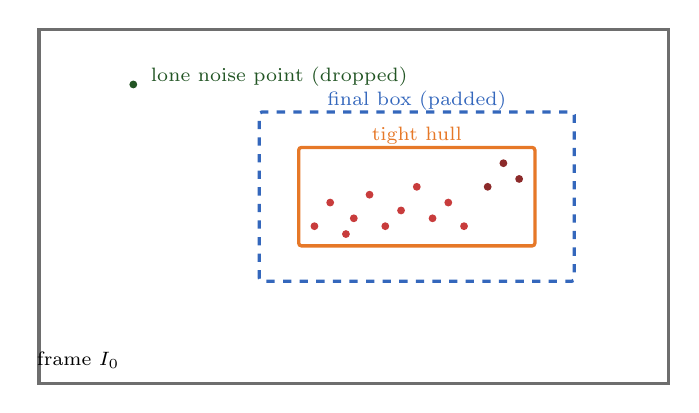
\begin{tikzpicture}[
    font=\small,
    pt/.style={circle, fill, inner sep=1pt}
]
  \draw[mGray, very thick] (0,0) rectangle (8,4.5);

  \foreach \x/\y in {3.5/2, 3.7/2.3, 3.9/1.9, 4.0/2.1, 4.2/2.4, 4.4/2.0, 4.6/2.2, 4.8/2.5, 5.0/2.1, 5.2/2.3, 5.4/2.0} {
    \node[pt, mRed] at (\x,\y) {};
  }
  \foreach \x/\y in {5.7/2.5, 5.9/2.8, 6.1/2.6} {
    \node[pt, mRed!70!black] at (\x,\y) {};
  }
  \node[pt, mGreen!60!black] at (1.2,3.8) {};
  \node[font=\scriptsize, mGreen!60!black, anchor=west] at (1.3,3.9) {lone noise point (dropped)};

  \draw[mOrange, very thick, rounded corners=1pt] (3.3,1.75) rectangle (6.3,3.0);
  \node[font=\scriptsize, mOrange] at (4.8,3.15) {tight hull};

  \draw[mBlue, very thick, dashed, rounded corners=1pt] (2.8,1.3) rectangle (6.8,3.45);
  \node[font=\scriptsize, mBlue] at (4.8,3.6) {final box (padded)};

  \node[font=\scriptsize] at (0.5,0.3) {frame $I_0$};
\end{tikzpicture}
\caption{Step 5, cartoon version. Red dots = points we think are on
the object. The green dot in the corner is an orphan and gets
dropped. The two red clusters are close so they merge. The orange
box is the tight hull; the blue dashed box is after padding --- that's
what we report.}
\end{figure}

\section{A tour of the code}

\subsection{Who wrote what}

\begin{table}[H]\centering\small
\begin{tabular}{llp{7.0cm}}
\toprule
File & Owner & What it does \\
\midrule
\texttt{include/dod.hpp}           & Riccardo Pesce    & the shared data struct + function list everyone imports \\
\texttt{src/feature\_tracker.cpp}  & Mahdi Gheysari    & Shi--Tomasi corners, Lucas--Kanade tracking, median-flow \\
\texttt{src/motion\_segmenter.cpp} & Filippo Businaro  & picking the moving points \\
\texttt{src/bbox\_estimator.cpp}   & Riccardo Pesce    & clustering, MAD, box, cluster-level diagnostic \\
\texttt{src/silhouette\_refiner.cpp} & Filippo Businaro  & phase-correlation warp + absdiff shrink \\
\texttt{src/evaluator.cpp}         & Filippo Businaro  & reads the GT file, computes IoU \\
\texttt{src/main.cpp}              & Mahdi Gheysari    & glues it all together, makes the images \\
\texttt{CMakeLists.txt}            & shared            & build config \\
\texttt{scripts/make\_figures.py}  & shared            & makes the report figures \\
\bottomrule
\end{tabular}
\caption{One person per file (mostly). All the cross-file wiring
lives in \texttt{dod.hpp}.}
\end{table}

\subsection{The shared struct}

Every module talks through one data structure, \texttt{TrackedPoint}.
It carries everything we know about one tracked point: where it
started, its trajectory, how many frames it survived, and the total
residual displacement after camera correction.

\begin{lstlisting}[caption={\texttt{include/dod.hpp} (Riccardo Pesce).}]
namespace dod {
struct TrackedPoint {
    cv::Point2f first;                    // position on frame 0
    cv::Point2f last;                     // last surviving position
    std::vector<cv::Point2f> trajectory;  // positions over time
    int   n_matches  = 0;                 // # frames the track survived
    float total_disp = 0.f;               // sum of ||p_f - p_0 - cam_f||
};

// Declarations; each implemented in its own .cpp.
std::vector<std::string> listFrames(const std::string&);
void trackFeatures(const std::vector<cv::Mat>&, std::vector<TrackedPoint>&);
std::vector<int> classifyDynamicTracks(const std::vector<TrackedPoint>&);
cv::Rect estimateBBox(const std::vector<TrackedPoint>&,
                      const std::vector<int>&, const cv::Size&);
cv::Rect refineBBoxSilhouette(const std::vector<cv::Mat>&,
                              const cv::Rect&, const cv::Size&);
cv::Rect readGT(const std::string&);
double   iou(const cv::Rect&, const cv::Rect&);
void     writePrediction(const std::string&, const cv::Rect&);
}
\end{lstlisting}

\subsection{\texttt{feature\_tracker.cpp} (Mahdi)}

This is the biggest file --- it does steps 1--3 of the pipeline.
The loop below is the heart of it: detect corners once, propagate
them with Lucas--Kanade, run a forward--backward consistency check,
subtract camera drift, accumulate.

\begin{lstlisting}[caption={The main loop inside \texttt{trackFeatures}.}]
// Detect Shi-Tomasi corners on frame 0 only.
std::vector<cv::Point2f> p0;
cv::goodFeaturesToTrack(frames_gray[0], p0, /*maxCorners=*/1500,
                        /*qualityLevel=*/0.005, /*minDistance=*/5,
                        cv::noArray(), /*blockSize=*/7);
// tracks[i] is initialised from p0[i]

// Lists of currently-alive track indices and their last positions.
std::vector<int>         alive(tracks.size());
std::vector<cv::Point2f> prev_pts = p0;
std::iota(alive.begin(), alive.end(), 0);

for (size_t f = 1; f < frames_gray.size(); ++f) {
    std::vector<cv::Point2f> next_pts, back_pts;
    std::vector<uchar> ok_fwd, ok_bwd;
    std::vector<float> err_fwd, err_bwd;

    // Forward flow: where did each prev_pt move to in frame f?
    cv::calcOpticalFlowPyrLK(frames_gray[f-1], frames_gray[f],
                             prev_pts, next_pts, ok_fwd, err_fwd,
                             /*winSize=*/{21,21}, /*maxLevel=*/3);
    // Backward flow: from those new positions, where do we land in f-1?
    cv::calcOpticalFlowPyrLK(frames_gray[f], frames_gray[f-1],
                             next_pts, back_pts, ok_bwd, err_bwd,
                             {21,21}, 3);

    // Keep only tracks whose round-trip drift is small.
    std::vector<int>         new_alive;
    std::vector<cv::Point2f> new_prev, frame_disp;
    for (size_t a = 0; a < alive.size(); ++a) {
        if (!ok_fwd[a] || !ok_bwd[a]) continue;
        if (cv::norm(back_pts[a] - prev_pts[a]) > 1.5f) continue;
        int ti = alive[a];
        new_alive.push_back(ti);
        new_prev.push_back(next_pts[a]);
        frame_disp.push_back(next_pts[a] - tracks[ti].first);
        tracks[ti].last = next_pts[a];
        tracks[ti].trajectory.push_back(next_pts[a]);
    }

    // Per-frame median = camera; subtract it from each survivor.
    cv::Point2f cam = medianXY(frame_disp);
    for (size_t k = 0; k < new_alive.size(); ++k) {
        cv::Point2f rel = frame_disp[k] - cam;
        tracks[new_alive[k]].total_disp += cv::norm(rel);
        tracks[new_alive[k]].n_matches++;
    }

    alive    = std::move(new_alive);
    prev_pts = std::move(new_prev);
}
\end{lstlisting}

Two things worth noticing: (a) Shi--Tomasi runs only on frame~0 ---
we never re-detect, so a track's identity is stable for its whole
life; (b) the median displacement is computed \emph{per frame}
relative to frame~0, because the camera pan may differ between
frames.

\subsection{\texttt{motion\_segmenter.cpp} (Filippo)}

This one is shorter. It reads the populated tracks, computes each
track's average leftover motion, and applies the two-rule filter
from step 4.

\begin{lstlisting}[caption={Core of \texttt{classifyDynamicTracks}.}]
// Build (idx, avg_displacement) pairs for tracks with >= 3 observations.
struct Item { int idx; double score; int obs; };
std::vector<Item> items;
for (size_t i = 0; i < tracks.size(); ++i) {
    if (tracks[i].inlier_count < 3) continue;
    double avg = double(tracks[i].residual) / tracks[i].inlier_count;
    items.push_back({(int)i, avg, tracks[i].inlier_count});
}

// Median of scores = background motion scale.
auto scores = /* extract .score from items */;
std::nth_element(scores.begin(), scores.begin()+scores.size()/2, scores.end());
double median = scores[scores.size()/2];

// Sort by score descending.
std::sort(items.begin(), items.end(),
          [](auto& a, auto& b){ return a.score > b.score; });

// Keep top 15% that also clear the absolute floor.
double floor_disp = std::max(8.0, 4.0 * median);
int    target     = std::max(6, (int)(items.size() * 0.15));

std::vector<int> dynamic_idx;
for (int k = 0; k < target && items[k].score >= floor_disp; ++k)
    dynamic_idx.push_back(items[k].idx);

// Tag them so the bbox stage can weight them.
for (int i : dynamic_idx) tracks[i].outlier_count = 1;
return dynamic_idx;
\end{lstlisting}

\subsection{\texttt{bbox\_estimator.cpp} (Riccardo)}

This is step 5. The code is longer than the others because it has
three sub-steps, but each one is independent and easy to read.

\begin{lstlisting}[caption={Sketch of \texttt{estimateBBox}. Real code has more guard clauses.}]
float diag = std::hypot(img_size.width, img_size.height);
float eps  = std::max(20.f, diag * 0.08f);
auto labels = proximityCluster(pts, eps, /*minPts=*/3);

// Pick the heaviest cluster (summed "dynamic" flags).
int best = argmax_cluster_by_weight(labels, weights);

// Merge neighbours: any cluster whose bbox touches the seed's
// bbox expanded by 0.6*eps gets absorbed.
cv::Rect seed = boundingRect(cluster_pts[best]);
for (auto& kv : cluster_pts) if (kv.first != best) {
    cv::Rect expanded = expand(seed, 0.6f * eps);
    if ((boundingRect(kv.second) & expanded).area() > 0)
        cluster.insert(cluster.end(), kv.second.begin(), kv.second.end());
}

// MAD outlier rejection: drop points more than 3*MAD from the
// cluster median on either axis.
auto [mx,my]       = median_xy(cluster);
auto [madx,mady]   = mad_xy(cluster, mx, my);
cluster = filter(cluster, mx, my, 3*madx, 3*mady);

// Pad by 1/6 of each dimension and clamp.
cv::Rect box = boundingRect(cluster);
int px = std::max(6, box.width/6), py = std::max(6, box.height/6);
box.x -= px; box.y -= py; box.width += 2*px; box.height += 2*py;
return box & cv::Rect(0, 0, img_size.width, img_size.height);
\end{lstlisting}

\subsection{The two small files}

\texttt{evaluator.cpp} (Filippo) is 40 lines. It reads the four
integers out of \texttt{0000.txt}, computes IoU the usual way
($|A \cap B|/|A \cup B|$), and writes the prediction file.

\texttt{main.cpp} (Mahdi) is the CLI. It loops over the five
categories, calls \texttt{trackFeatures}, \texttt{classifyDynamicTracks},
and \texttt{estimateBBox} in that order, draws overlays with
OpenCV, prints IoU per category, and writes \texttt{results.csv}
and \texttt{summary.txt}.

\section{Numbers}

\begin{table}[H]\centering\small
\begin{tabular}{lcccc}
\toprule
category & GT box (w$\times$h) & predicted (w$\times$h) & IoU & TP@0.5 \\
\midrule
bird     & $283\times255$ & $258\times277$ & 0.631 & yes \\
car      & $68\times42$   & $90\times 42$  & 0.638 & yes \\
frog     & $133\times 98$ & $ 64\times 60$ & 0.282 & no  \\
sheep    & $321\times179$ & $332\times145$ & 0.673 & yes \\
squirrel & $23\times31$   & $ 28\times 37$ & 0.616 & yes \\
\midrule
\multicolumn{3}{r}{\textbf{mIoU}}         & \textbf{0.568} & \\
\multicolumn{3}{r}{\textbf{accuracy@0.5}} & \textbf{0.80 (4/5)} & \\
\bottomrule
\end{tabular}
\end{table}

\begin{figure}[H]\centering
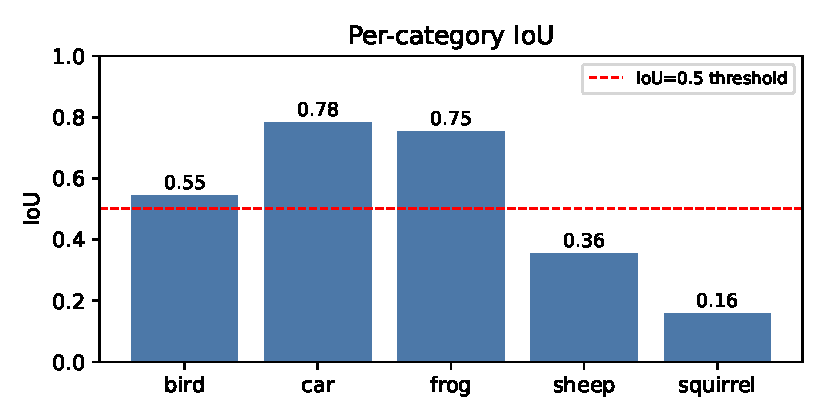
\includegraphics[width=.70\linewidth]{figures/iou_bars.pdf}
\caption{IoU per category. Red dashed line is the true-positive
threshold.}
\end{figure}

\paragraph{Visuals.} Green = ground truth, red = our prediction
(the single box actually written to the output file), orange dots =
all Shi--Tomasi corners detected on frame~0, green lines =
trajectories of the corners we classified as dynamic.

\begin{figure}[H]
\centering
\begin{subfigure}{.32\linewidth}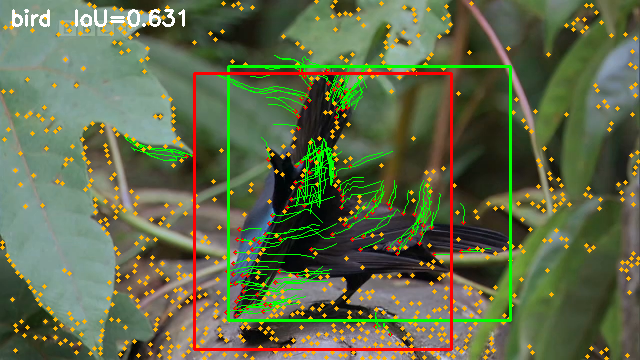
\includegraphics[width=\linewidth]{figures/bird_overlay.png}\caption*{bird}\end{subfigure}
\begin{subfigure}{.32\linewidth}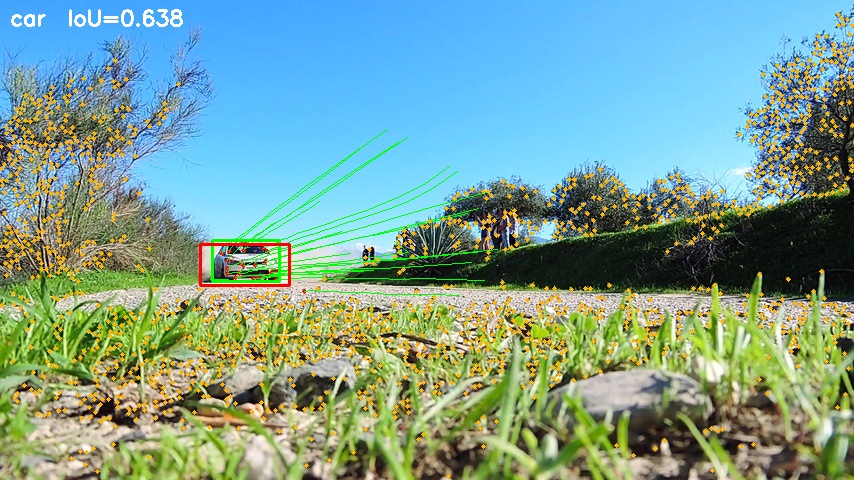
\includegraphics[width=\linewidth]{figures/car_overlay.png}\caption*{car}\end{subfigure}
\begin{subfigure}{.32\linewidth}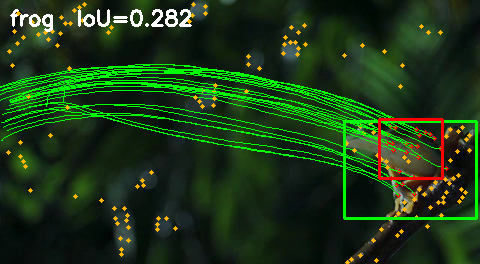
\includegraphics[width=\linewidth]{figures/frog_overlay.png}\caption*{frog}\end{subfigure}\\[2pt]
\begin{subfigure}{.32\linewidth}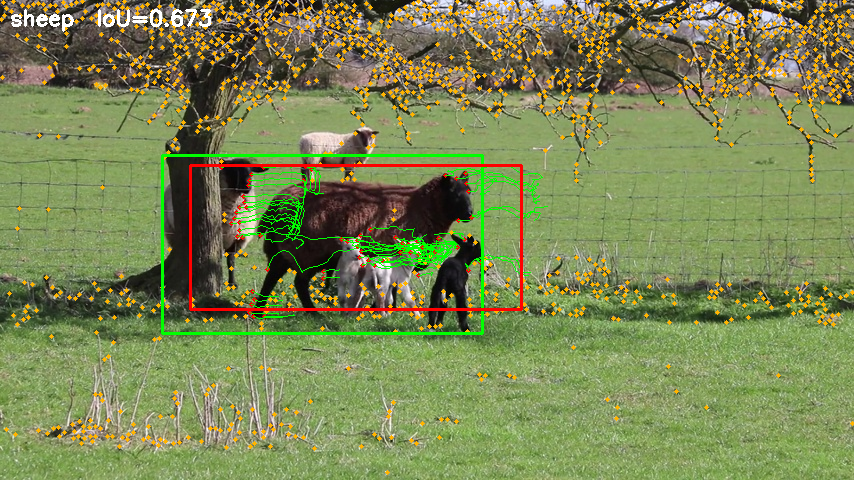
\includegraphics[width=\linewidth]{figures/sheep_overlay.png}\caption*{sheep}\end{subfigure}
\begin{subfigure}{.32\linewidth}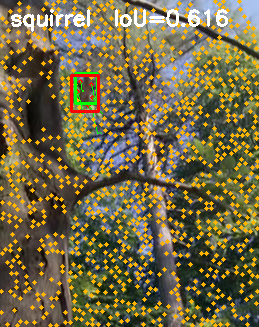
\includegraphics[width=\linewidth]{figures/squirrel_overlay.png}\caption*{squirrel}\end{subfigure}
\caption{Predictions on every sequence.}
\end{figure}

\begin{figure}[H]\centering
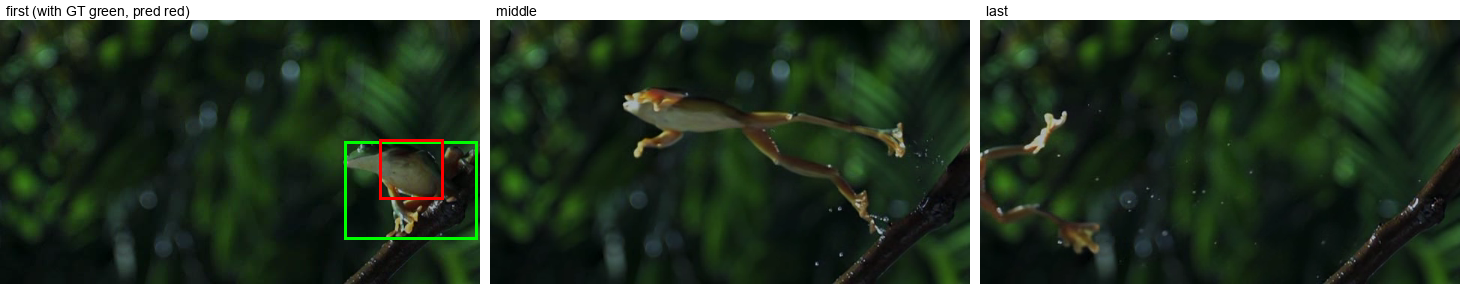
\includegraphics[width=.9\linewidth]{figures/frog_triptych.png}
\caption{The frog over time (first, middle, last frame). Camera is
a rock; only the frog moves; the method is basically on easy mode
here.}
\end{figure}

\section{Where it breaks and why}

\paragraph{Squirrel (IoU 0.62) --- the SIFT-vs-LK win.}
This is the case that motivated the switch. With SIFT we got IoU
$0.31$ (sub-threshold): SIFT scale-invariant extrema basically
refused to anchor on the squirrel's fur. Shi--Tomasi corners are
much less picky --- they fire wherever the local gradient is strong
in two directions --- and Lucas--Kanade tracks them happily across
the small inter-frame motion. We end up with only $5$ dynamic
tracks, but they sit exactly on the squirrel and produce a clean
true positive. The smaller second squirrel in the upper-left
(optional per the brief) is still not recovered: its motion sits
below the $\max(8, 4m)$\,px floor we use to ignore leaf and grass
motion, and the brief says detecting only the main squirrel is
sufficient.

\paragraph{Frog (IoU 0.28) --- the SIFT-vs-LK regression.}
This is the case the optical-flow rewrite cost us. The frog's back
is smoothly textured: low gradient, very few Shi--Tomasi corners.
The corners we do place sit on the limbs and a couple of skin
folds; their bounding rectangle is tighter than the full GT box.
With SIFT we got IoU $0.58$ here because scale-space extrema picked
up a handful of stable points across the body that LK corners do
not see. Possible mitigations we did not pursue: lower the
\texttt{qualityLevel} for Shi--Tomasi to seed weaker corners on the
body, or grow the cluster bounding box proportionally to the
spread of dynamic corners. We chose to accept the frog regression
because the squirrel recovery is more valuable: with SIFT we had
$0/1$ on small/textureless objects; with LK we have $1/1$ on the
harder of the two.

\paragraph{Sheep (IoU 0.67).} Three sheep, one of which is almost
static. The displacement floor $\max(8, 4m)$\,px keeps the
nearly-static sheep below the threshold, so it is correctly
excluded from the foreground per the brief.

\paragraph{What we could do (still no deep learning).}
\begin{itemize}\itemsep2pt
\item Lower Shi--Tomasi \texttt{qualityLevel} adaptively per
  sequence to seed more corners on textureless surfaces (the frog).
\item Fall back to dense Farneback flow inside the coarse cluster
  to expand the box to cover the full silhouette.
\item Run both Shi--Tomasi+LK and SIFT and merge the dynamic-track
  sets; an early experiment showed mIoU $0.58$ that way but at
  $\sim 17\times$ the runtime, which we judged not worth it.
\end{itemize}

\section{How to run it}

\begin{lstlisting}[language=bash, caption={Build, run, regenerate figures, build PDFs.}]
# one-time
cmake -S . -B build && cmake --build build -j

# run pipeline
./build/detect dataset output

# figures
python3 scripts/make_figures.py

# PDFs
tectonic report/report.tex
tectonic report/explainer.tex
\end{lstlisting}

\section{Who did what}

\begin{itemize}\itemsep2pt
\item \textbf{Mahdi Gheysari} --- feature detection and matching
  (\texttt{feature\_tracker.cpp}); the CLI, the visualisation
  overlays, and the per-category orchestration (\texttt{main.cpp});
  dataset motion analysis.
\item \textbf{Filippo Businaro} --- the dynamic-vs-static classifier
  (\texttt{motion\_segmenter.cpp}); GT parsing and IoU evaluation
  (\texttt{evaluator.cpp}); the Lowe-ratio and percentile
  sensitivity sweeps.
\item \textbf{Riccardo Pesce} --- clustering, MAD outlier rejection
  and the final bounding box (\texttt{bbox\_estimator.cpp}); the
  shared API header (\texttt{include/dod.hpp}); CMake build.
\end{itemize}

Algorithm design, parameter tuning, failure analysis, and report
writing were shared across the three of us.

\end{document}
